\section{Cell Tracking}

\begin{frame}{Cell Tracking - Requirements}
    \begin{figure}
        \centering
        \begin{tikzpicture}
            \begin{scope}[baseline=(image1.south)]
                \node[label=above:$t$] (image1) {
                    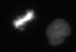
\includegraphics[width=0.25\textwidth]{images/cell_tracking/example_00.png}
                };
                \uncover<2->{
                    \node[transparent_node, red, xshift=-12pt, yshift=5pt] (d11) at (image1.center) {}; 
                    \node[transparent_node, green, xshift=20pt, yshift=-5pt] (d12) at (image1.center) {}; 
                }
            \end{scope}
            \begin{scope}[baseline=(image2.south)]
                \node[right=of image1, xshift=-20pt, label=above:$t+1$] (image2) {
                    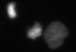
\includegraphics[width=0.25\textwidth]{images/cell_tracking/example_01.png}
                };
                \uncover<3->{
                    \node[transparent_node, red, xshift=-25pt, yshift=15pt] (d21) at (image2.center) {}; 
                    \node[transparent_node, red, xshift=0pt, yshift=-5pt] (d22) at (image2.center) {};
                    \node[transparent_node, green, xshift=18pt, yshift=-10pt] (d23) at (image2.center) {};
                    \path[assignment_arrow, red, bend left=20] (d11) edge (d21);
                    \path[assignment_arrow, red, bend left=10] (d11) edge (d22);
                    \path[assignment_arrow, green, bend right=20] (d12) edge (d23.south west);
                }
            \end{scope}
            \begin{scope}[baseline=(image3.south)]
                \node[right=of image2, xshift=-20pt, label=above:$t+2$] (image3) {
                    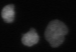
\includegraphics[width=0.25\textwidth]{images/cell_tracking/example_02.png}
                };
                \uncover<4->{
                    \node[transparent_node, red, xshift=-26pt, yshift=13pt] (d31) at (image3.center) {}; 
                    \node[transparent_node, red, xshift=-7pt, yshift=-13pt] (d32) at (image3.center) {};
                    \node[transparent_node, green, xshift=18pt, yshift=-8pt] (d33) at (image3.center) {}; 
                    \path[assignment_arrow, red, bend left=20] (d21) edge (d31);
                    \path[assignment_arrow, red, bend left=20] (d22.north east) edge (d32);
                    \path[assignment_arrow, green, bend right=35] (d23.south east) edge (d33.south west);
                }
            \end{scope}
        \end{tikzpicture}
    \end{figure}
            
    \begin{itemize}
          \item Extract cell lineages from embryo data.
          \item Reconstruct fates of all cells in the embryo.
          \item Applicable in 2D and 3D.
    \end{itemize}
\end{frame}

% \begin{frame}{Existing Work}
%     Two approache:s
%     \begin{enumerate}
%           \item State space models.
%           \item Tracking-by-Assignment
%         \begin{itemize}
%               \item Chain Graph Tracking
%         \end{itemize}
%     \end{enumerate}
% \end{frame}

\begin{frame}{Tracking-by-Assignment}
    \begin{figure}
        \centering
        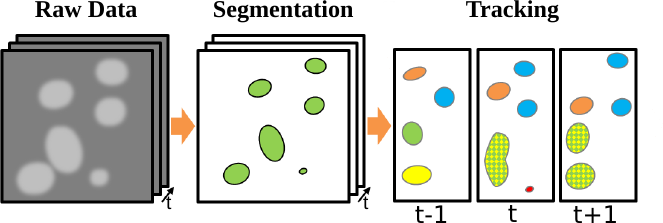
\includegraphics[width=\textwidth]{images/cell_tracking/pipeline_mod.png}
        \caption{Chain graph tracking pipeline [SOURCE].}
        \label{fig:chaingraph-pipeline}
    \end{figure}
\end{frame}

\begin{frame}{Hypotheses Graph}
    % \begin{figure}
    \begin{center}
        \only<1>{
            % \begin{subfigure}[b]{0.44\textwidth}
            %     \centering
                \scalebox{0.62}{
                    \begin{tikzpicture}[minimum size=58pt,scale=0.45, every node/.style={scale=0.45, text=black, font=\LARGE}, thick]
                            \begin{scope}
        \node (t1) {\huge $t$};
        \node[hypothesesdetection, below=of t1, circle, draw] (x11) {$X_1^t$};
        \node[hypothesesdetection, below=of x11, circle, draw] (x12) {$X_2^t$};
        \node[hypothesesdetection, below=of x12, circle, draw] (x13) {$X_3^t$};
    \end{scope}

    
    
    \begin{scope}
        \node[right=of t1, xshift=15mm] (t2) {\huge $t+1$};
        \node[hypothesesdetection, below=of t2, circle, draw] (x21) {$X_4^{t+1}$};
        \node[hypothesesdetection, below=of x21, circle, draw] (x22) {$X_5^{t+1}$};
    \end{scope}

    \begin{scope}[on background layer]
        \node[hypothesesdetection, below=of x22, circle, draw, on background layer] (x23) {$X_6^{t+1}$};
    \end{scope}
    
    
    \begin{scope}
        \node[right=of t2, xshift=15mm] (t3) {\huge $t+2$};
        \node[hypothesesdetection, below=of t3, circle, draw] (x31) {$X_7^{t+2}$};
        \node[hypothesesdetection, circle, draw, shift=($(x31.center)-(x21.center)$)] (x32) at (x22) {$X_8^{t+2}$};
    \end{scope}
    
    \begin{scope}[on background layer]
        \node[hypothesesdetection, below=of x32, circle, draw, on background layer] (x33) {$X_{10}^{t+2}$};
    \end{scope}
    
    % \begin{scope}
    %     \node[right=of t3, xshift=15mm] (t4) {\huge $t+3$};
    %     \node[hypothesesdetection, below=of t4, circle, draw] (x41) {$X_{10}^{t+3}$};
    %     \node[hypothesesdetection, below=of x41, circle, draw] (x42) {$X_{11}^{t+3}$};
    %     \node[hypothesesdetection, below=of x42, circle, draw] (x43) {$X_{12}^{t+3}$};
    % \end{scope}

    \begin{scope}[on background layer]
        \node[rectangle, draw, color=hypothesesbackground!40, fill=hypothesesbackground!30,
        fit=(x11) (x12) (x13), inner sep=13mm] (b1) {};
        \node[rectangle, draw, color=hypothesesbackground!40, fill=hypothesesbackground!30,
        fit=(x21) (x22) (x23), inner sep=13mm] (b2) {};
        \node[rectangle, draw, color=hypothesesbackground!40, fill=hypothesesbackground!30,
        fit=(b2), shift=($(t3.center) - (t2.center)$), inner sep=-0.1mm] (b3) {};
        % \node[rectangle, draw, color=hypothesesbackground!40, fill=hypothesesbackground!30,
        % fit=(x41) (x42) (x43), inner sep=13mm] (b4) {};
    \end{scope}

    \path[hypothesestransition] (x11) edge (x21);
    \path[hypothesestransition] (x12) edge (x22);
    \path[hypothesestransition] (x13) edge (x22);
    % \path[hypothesestransition] (x13) edge (x23);

    \path[hypothesestransition] (x21) edge (x31);
    \path[hypothesestransition] (x21) edge (x32);
    \path[hypothesestransition] (x22) edge (x32);
    % \path[hypothesestransition] (x23) edge (x32);

    % \path[hypothesestransition] (x31) edge (x41);
    % \path[hypothesestransition] (x32) edge (x42);
    % \path[hypothesestransition] (x32) edge (x43);

%%% Local Variables: 
%%% mode: latex
%%% TeX-master: "../../../main"
%%% End: 



%%% Local Variables: 
%%% mode: latex
%%% TeX-master: "../../main"
%%% End: 

                    \end{tikzpicture}
                }
            % \end{subfigure}
        }
        % \hfill
        \only<2>{
            % \begin{subfigure}[b]{0.44\textwidth}
            %     \centering
                \scalebox{0.62}{
                    \begin{tikzpicture}[minimum size=58pt,scale=0.45, every node/.style={scale=0.45, text=black, font=\LARGE}, thick]
                            \begin{scope}
        \node (t1) {\huge $t$};
        \node[hypothesesdetection, below=of t1, circle, draw] (x11) {$X_1^t$};
    \end{scope}
    \begin{scope}[on background layer]
        \node[hypothesesdetection, below=of x11, circle, draw] (x12) {$X_2^t$};
    \end{scope}
    \begin{scope}
        \node[hypothesesdetection, below=of x12, circle, draw] (x13) {$X_3^t$};
    \end{scope}

    
    
    \begin{scope}
        \node[right=of t1, xshift=15mm] (t2) {\huge $t+1$};
        \node[hypothesesdetection, below=of t2, circle, draw] (x21) {$X_4^{t+1}$};
        \node[hypothesesdetection, below=of x21, circle, draw] (x22) {$X_5^{t+1}$};
    \end{scope}

    \begin{scope}[on background layer]
        \node[hypothesesdetection, below=of x22, circle, draw, on background layer] (x23) {$X_6^{t+1}$};
    \end{scope}
    
    
    \begin{scope}
        \node[right=of t2, xshift=15mm] (t3) {\huge $t+2$};
        \node[hypothesesdetection, below=of t3, circle, draw] (x31) {$X_7^{t+2}$};
        \node[hypothesesdetection, circle, draw, shift=($(x31.center)-(x21.center)$)] (x32) at (x22) {$X_8^{t+2}$};
    \end{scope}
    
    \begin{scope}[on background layer]
        \node[hypothesesdetection, below=of x32, circle, draw, on background layer] (x33) {$X_{10}^{t+2}$};
    \end{scope}
    
    % \begin{scope}
    %     \node[right=of t3, xshift=15mm] (t4) {\huge $t+3$};
    %     \node[hypothesesdetection, below=of t4, circle, draw] (x41) {$X_{10}^{t+3}$};
    %     \node[hypothesesdetection, below=of x41, circle, draw] (x42) {$X_{11}^{t+3}$};
    %     \node[hypothesesdetection, below=of x42, circle, draw] (x43) {$X_{12}^{t+3}$};
    % \end{scope}

    \begin{scope}[on background layer]
        \node[rectangle, draw, color=hypothesesbackground!40, fill=hypothesesbackground!30,
        fit=(x11) (x12) (x13), inner sep=13mm] (b1) {};
        \node[rectangle, draw, color=hypothesesbackground!40, fill=hypothesesbackground!30,
        fit=(x21) (x22) (x23), inner sep=13mm] (b2) {};
        \node[rectangle, draw, color=hypothesesbackground!40, fill=hypothesesbackground!30,
        fit=(b2), shift=($(t3.center) - (t2.center)$), inner sep=-0.1mm] (b3) {};
        % \node[rectangle, draw, color=hypothesesbackground!40, fill=hypothesesbackground!30,
        % fit=(x41) (x42) (x43), inner sep=13mm] (b4) {};
    \end{scope}

    \path[hypothesestransition] (x11) edge (x21);
    % \path[hypothesestransition] (x12) edge (x22);
    \path[hypothesestransition] (x13) edge (x22);
    % \path[hypothesestransition] (x13) edge (x23);

    \path[hypothesestransition] (x21) edge (x31);
    % \path[hypothesestransition] (x21) edge (x32);
    \path[hypothesestransition] (x22) edge (x32);
    % \path[hypothesestransition] (x23) edge (x32);

    % \path[hypothesestransition] (x31) edge (x41);
    % \path[hypothesestransition] (x32) edge (x42);
    % \path[hypothesestransition] (x32) edge (x43);

%%% Local Variables: 
%%% mode: latex
%%% TeX-master: "../../../main"
%%% End: 



%%% Local Variables: 
%%% mode: latex
%%% TeX-master: "../../main"
%%% End: 

                    \end{tikzpicture}
                }
            % \end{subfigure}
            }
        \end{center}
    %     \caption{Hypotheses Graph for potential detections and assignments.}
    %     \label{fig:cell-tracking-hypotheses}
    % \end{figure}
\end{frame}



% \begin{frame}{Chain Graph Tracking}
%     \begin{figure}
%         \centering
%         \begin{subfigure}[b]{0.44\textwidth}
%             \centering
%             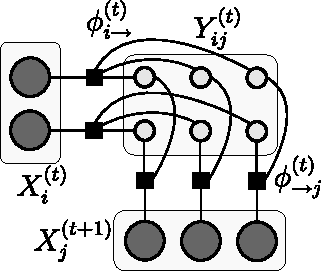
\includegraphics[width=\textwidth]{images/cell_tracking/fig_crf_less_nodes.pdf}
%             \caption{CRF}
%             \label{fig:chaingraph-crf}
%         \end{subfigure}
%         \hspace{5pt}
%         \begin{subfigure}[b]{0.44\textwidth}
%             \centering
%             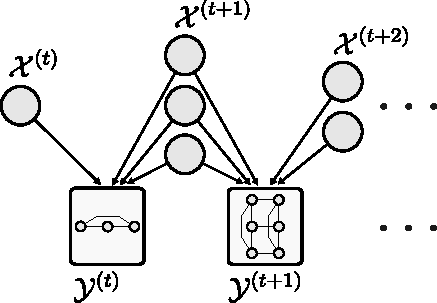
\includegraphics[width=\textwidth]{images/cell_tracking/fig_chain_graph.pdf}
%             \caption{Chain Graph}
%             \label{fig:chaingraph-cg}
%         \end{subfigure}
%         \caption{Chain graph model. [SOURCE]}
%         \label{fig:chaingraph-model}
%     \end{figure}
% \end{frame}

% \begin{frame}{Chain Graph Tracking}
%     to be discussed
%     \begin{itemize}
%           \item Can distinguish between cells and noise.
%           \item Allows for tracking in oversegmented images.
%           \item Fails in case of undersegmentation, that is in the presence of merged or overlapping objects.
%     \end{itemize}
%     [Kausler \etal (2012)] REFERENZ
% \end{frame}


%%% Local Variables: 
%%% mode: latex
%%% TeX-master: "../main"
%%% End: 
